\documentclass{article}
\usepackage[utf8]{inputenc}

%%% Packages %%%
\usepackage[margin=1in]{geometry}
\usepackage{amsmath, amsthm, amssymb}
\usepackage[arrowmos, american voltages]{circuitikz}
\usepackage{enumitem}
\usepackage{fancyhdr} % for the top header
\usepackage{float}
\usepackage{fancyhdr}
\usepackage{graphicx}
\PassOptionsToPackage{hyphens}{url}\usepackage{hyperref} % allow for URL wrapping
\usepackage{lastpage} % just for last page
\usepackage{mathtools}
\usepackage[super]{nth}
\usepackage{physics}
\usepackage{siunitx} % nice units formatting
\usepackage{tikz}
\usepackage{verbatim}

% code env packages
\usepackage{listings, lstautogobble}
\usepackage{color}
\usepackage[T1]{fontenc}

\setlength\parindent{0pt}

%%% HEADERS %%%
\title{Newton's Approximation in Nonlinear Circuits}
\author{Michael You}
\date{January 30, 2019}

\fancyhf{}
\lhead{18-220: Newton's Approximation Method}
\rhead{}
\fancyfoot[C]{\thepage}

% Environments
\theoremstyle{definition}
\newtheorem{definition}{Definition}

%%% Custom math shortcuts %%%
\DeclarePairedDelimiter{\ceil}{\lceil}{\rceil}
\DeclarePairedDelimiter{\floor}{\lfloor}{\rfloor}
\DeclarePairedDelimiter{\paren}{(}{)}
\DeclarePairedDelimiter{\bracken}{[}{]}
\DeclarePairedDelimiter{\bracens}{\{}{\}}
\newcommand{\pa}[1]{\paren*{#1}}
\newcommand{\pbra}[1]{\bracken*{#1}}
\newcommand{\pbrc}[1]{\bracens*{#1}}
\newcommand{\db}[1]{\llbracket{#1}\rrbracket}
\newcommand{\bangle}[1]{\left\langle #1 \right\rangle}

%%% Useful shortcuts %%%
\newcommand{\te}[1]{\texttt{#1}} % for programming font
\newcommand{\eq}{=}
\newcommand{\ps}{\mathbin{\|}} % parallel resistors

% For transistor equations
\newcommand{\VG}{V_\text{G}}
\newcommand{\VS}{V_\text{S}}
\newcommand{\VD}{V_\text{D}}
\newcommand{\VGS}{V_\text{GS}}
\newcommand{\VDS}{V_\text{DS}}
\newcommand{\VTH}{V_\text{TH}}
\newcommand{\VDD}{V_\text{DD}}

%%% TODO Make \VI => \VIN to be consistent, same with \VOUT %%%
\newcommand{\VI}{V_\text{IN}}
\newcommand{\VIN}{V_\text{IN}}
\newcommand{\VO}{V_\text{OUT}}
\newcommand{\VOUT}{V_\text{OUT}}
\newcommand{\VDZ}{v_{\text{D}_0}}
\newcommand{\vt}{v_\text{T}}
\newcommand{\id}{i_\text{D}}
\newcommand{\vd}{v_\text{D}}

% SIUNITX
\sisetup{quotient-mode=fraction} % Output a/b as \frac{a}{b}

% tikz
\usetikzlibrary{decorations.pathreplacing}
\ctikzset{bipoles/resistor/height=0.2}
\ctikzset{bipoles/resistor/width=0.5}
\ctikzset{bipoles/diode/width=0.4}
\ctikzset{bipoles/diode/height=0.4}
\ctikzset{monopoles/ground/width=0.15}

%%% CODE ENV %%%

% colors
\definecolor{mygreen}{rgb}{0,0.6,0}
\definecolor{mygray}{rgb}{0.5,0.5,0.5}
\definecolor{mymauve}{rgb}{0.58,0,0.82}

% macro to select a scaled-down version of Bera Mono (for instance)
\makeatletter
\newcommand\BeraMonottfamily{%
  \def\fvm@Scale{0.78}% scales the font down
  \fontfamily{fvm}\selectfont% selects the Bera Mono font
}
\makeatother

\lstset{ 
  autogobble=true
  backgroundcolor=\color{white},   % choose the background color; you must add \usepackage{color} or \usepackage{xcolor}; should come as last argument
  basicstyle=\BeraMonottfamily,        % the size of the fonts that are used for the code
  breakatwhitespace=false,         % sets if automatic breaks should only happen at whitespace
  breaklines=true,                 % sets automatic line breaking
  captionpos=b,                    % sets the caption-position to bottom
  commentstyle=\color{mygreen},    % comment style
  columns=fullflexible,
  deletekeywords={...},            % if you want to delete keywords from the given language
  % escapeinside={\%*}{*)},          % if you want to add LaTeX within your code
  extendedchars=false,              % lets you use non-ASCII characters; for 8-bits encodings only, does not work with UTF-8
  frame=single,
  keepspaces=true,                 % keeps spaces in text, useful for keeping indentation of code (possibly needs columns=flexible)
  keywordstyle=\color{blue},       % keyword style
  % morekeywords={*,...},            % if you want to add more keywords to the set
  numbersep=5pt,                   % how far the line-numbers are from the code
  numberstyle=\footnotesize\color{mygray}\ttfamily, % the style that is used for the line-numbers
  rulecolor=\color{black},         % if not set, the frame-color may be changed on line-breaks within not-black text (e.g. comments (green here))
  showspaces=false,                % show spaces everywhere adding particular underscores; it overrides 'showstringspaces'
  showstringspaces=false,          % underline spaces within strings only
  showtabs=false,                  % show tabs within strings adding particular underscores
  stringstyle=\color{mymauve},     % string literal style
  tabsize=2,	                   % sets default tabsize to 2 spaces
  title=\lstname                   % show the filename of files included with \lstinputlisting; also try caption instead of title  
}

\pagestyle{fancy}

\begin{document}

\maketitle

With linear circuits, we can often get by pretty easily with Ohm's law, KVL, KCL, etc... 
But once we start talking about non-linear circuit elements, such as a diode, it seems
like we are at a lost for tools to use.

\section{The Problem}
Let's consider the following circuit

\begin{figure}[H]
  \centering

  \begin{circuitikz}
  % Drain
  \draw
  (0,0) node[left] {$\VIN$}
  to[short, *-] (1,0)
  to[D*, v=$\vd$] (3,0)
  to[R=$R \eq \SI{10}{\ohm}$] (5,0)
  node[sground, rotate=90] {};
  ;
  \end{circuitikz}
  \label{circuit}
\end{figure}

Suppose that
\begin{itemize}
  \item $\VIN = \SI{8}{\volt}$
  \item $\id = I_s\pa{e^{\vd/\vt} - 1}$, where $I_s = \SI{1e-24}{\ampere}$, $\vt = \SI{25}{\milli\volt}$
\end{itemize}

Solve for the current through the diode.

\section{A Na\"{i}ve Approach}
Hey, KCL works most of the time, so let's try it...

\begin{align*}
  \id &= \frac{\VIN - \vd}{R} \\
  I_s\pa{e^{\vd/\vt} - 1} &= \frac{\VIN - \vd}{R}\\
  I_se^{\vd/\vt} + \frac{\vd}{R} &= \frac{\VIN}{R} + I_s
\end{align*}

Oh man, it doesn't look like $\vd$ is easy to solve here...so what do we do here?

\clearpage
\section{Graph it!}
If you recall from Algebra, if we have two unknowns and two equations, we can find the intersection of the two curves to find their solution.
We don't know $\vd, \id$, and we have equations for each, so why not graph them?

\begin{figure}[H]
  \centering
  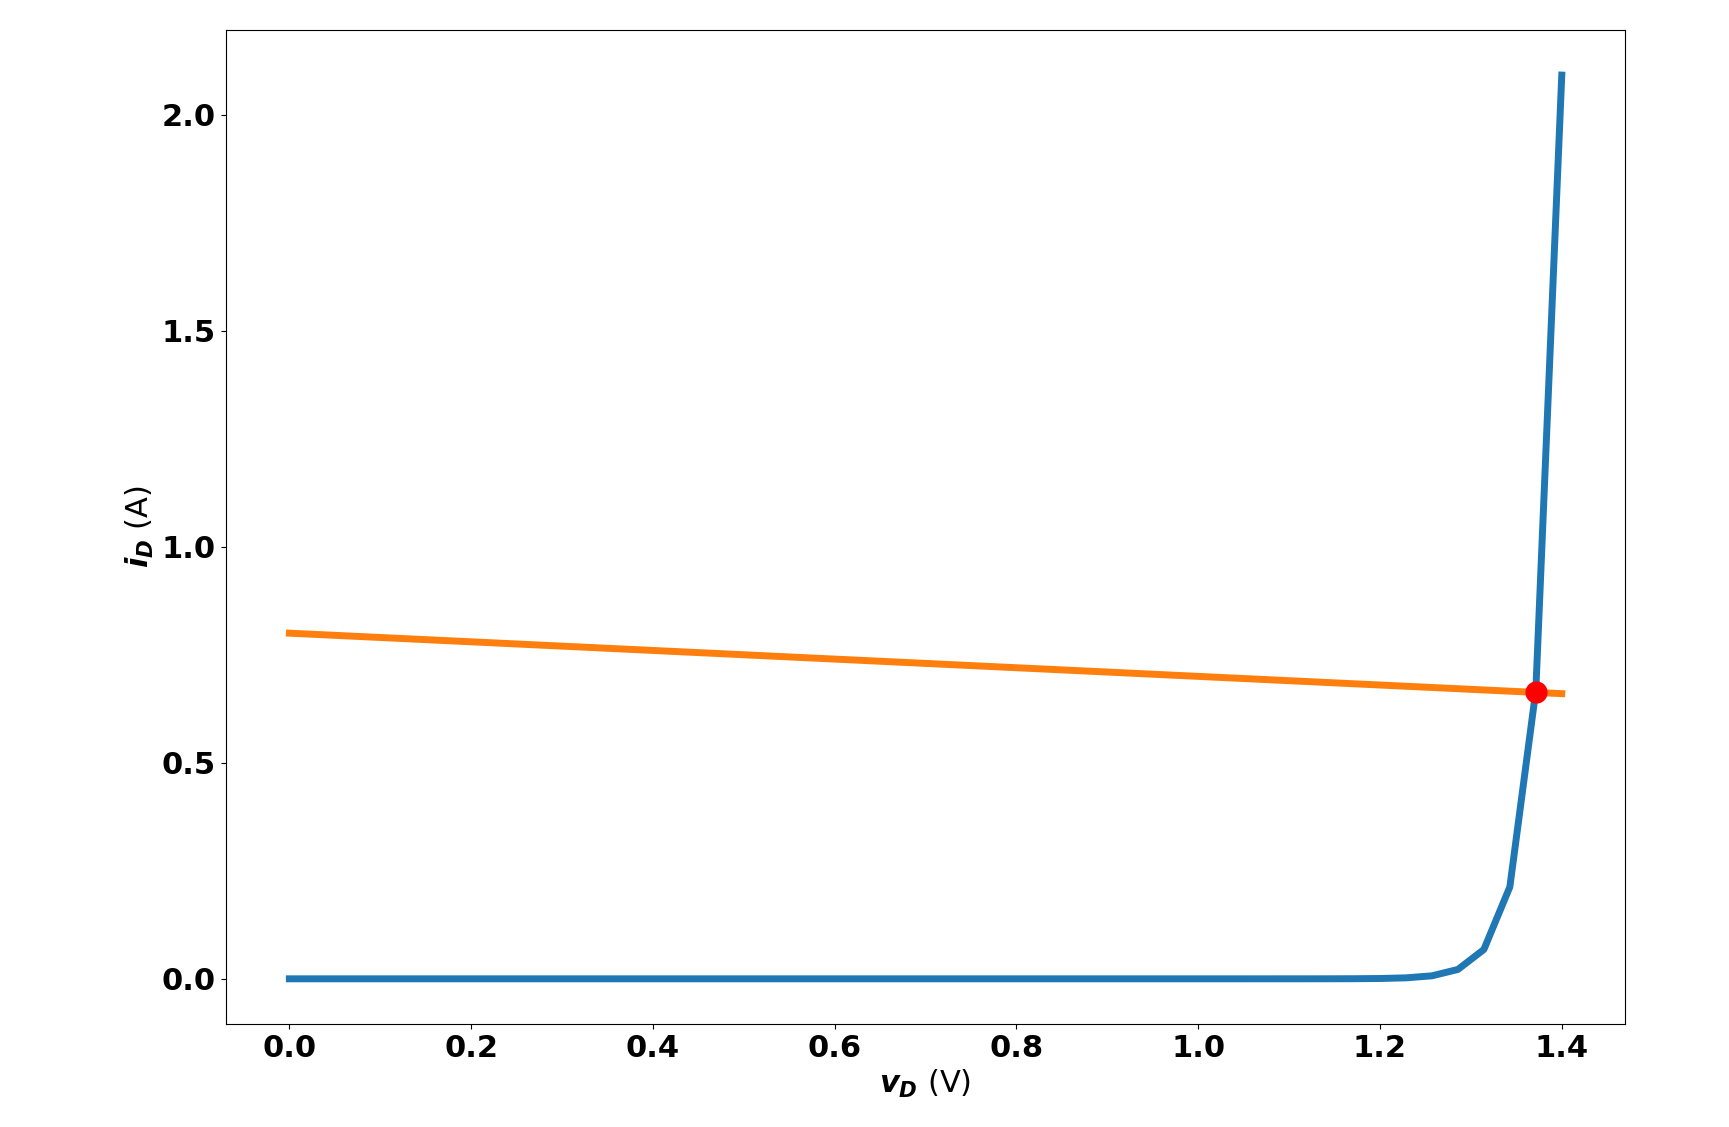
\includegraphics[height=3in]{plot.png}
\end{figure}

So yeah, this works pretty well, and we can find a solution at $(\vd, \id) = (\SI{1.371}{\volt}, \SI{0.663}{\ampere})$, 
but it can cause a lot of unnecessary strain on your calculator because it has to plot so many points.
In addition, how did the calculator find the points in the first place?

\clearpage
\section{Newton's Method}
In fact, even the calculator had to use some sort of numerical method to approximate the intersection of the two curves! 
One popular and fairly reliable method is:

\begin{definition}
  \textbf{Newton's Method} is a first-order numerical approximation method to estimate the root of a function.
  In particular, given 
  \begin{align}
    f(x) &= 0 \\
    x_0 &= \text{initial guess}
  \end{align}
  iterate
  \begin{equation}
    x_{n+1} = x_n - \frac{f(x_n)}{f'(x_n)}
  \end{equation}
  until $\abs{f(x_n)} < \epsilon$, for some sufficiently small $\epsilon > 0$ that defines the desired accuracy.
\end{definition}

For our problem, we can define
\begin{equation}
  f(\vd) = I_S\pa{
    e^{\vd/\vt} - 1
  } - \frac{
    \VIN - \vd
  }{
    R
  } = 0
\end{equation}

We also need the derivative, 

\begin{equation}
  \dv{f(\vd)}{\vd} = 
  \frac{I_S}{\vt}e^{\vd/\vt} 
  + \frac{1
  }{
    R
  }
\end{equation}

Now, we just need to iterate with the following iterative sequence:
\begin{equation}
  \begin{aligned}
    \VDZ &= v_{\text{D}_\text{initial}} \\
    v_{\text{D}_{i+1}} &= v_{\text{D}_i} - \frac{
      f(v_{\text{D}_i})
    }{
        f'(v_{\text{D}_i})
    }
  \end{aligned}
\end{equation}

Choosing an initial guess of $\VDZ = \SI{1.3}{\volt}$ gives us a final convergence value of
\begin{equation}
  \boxed{
    (\vd, \id) = (\SI{1.371}{\volt}, \SI{0.663}{\ampere})
  }
\end{equation}

\clearpage
\appendix
\section{Implementation of Newton's Method}
In Python because MATLAB is dying...

\lstinputlisting[language=Python]{newtons.py}

\end{document}